\documentclass[border=10pt]{standalone}
\usepackage[svgnames]{xcolor}
\usepackage{amsmath}
\usepackage{pgfplots}
\pgfplotsset{compat=newest}
\usepackage[sfdefault]{FiraSans}
\usepackage{FiraMono}
\renewcommand*\familydefault{\sfdefault}
\begin{document}
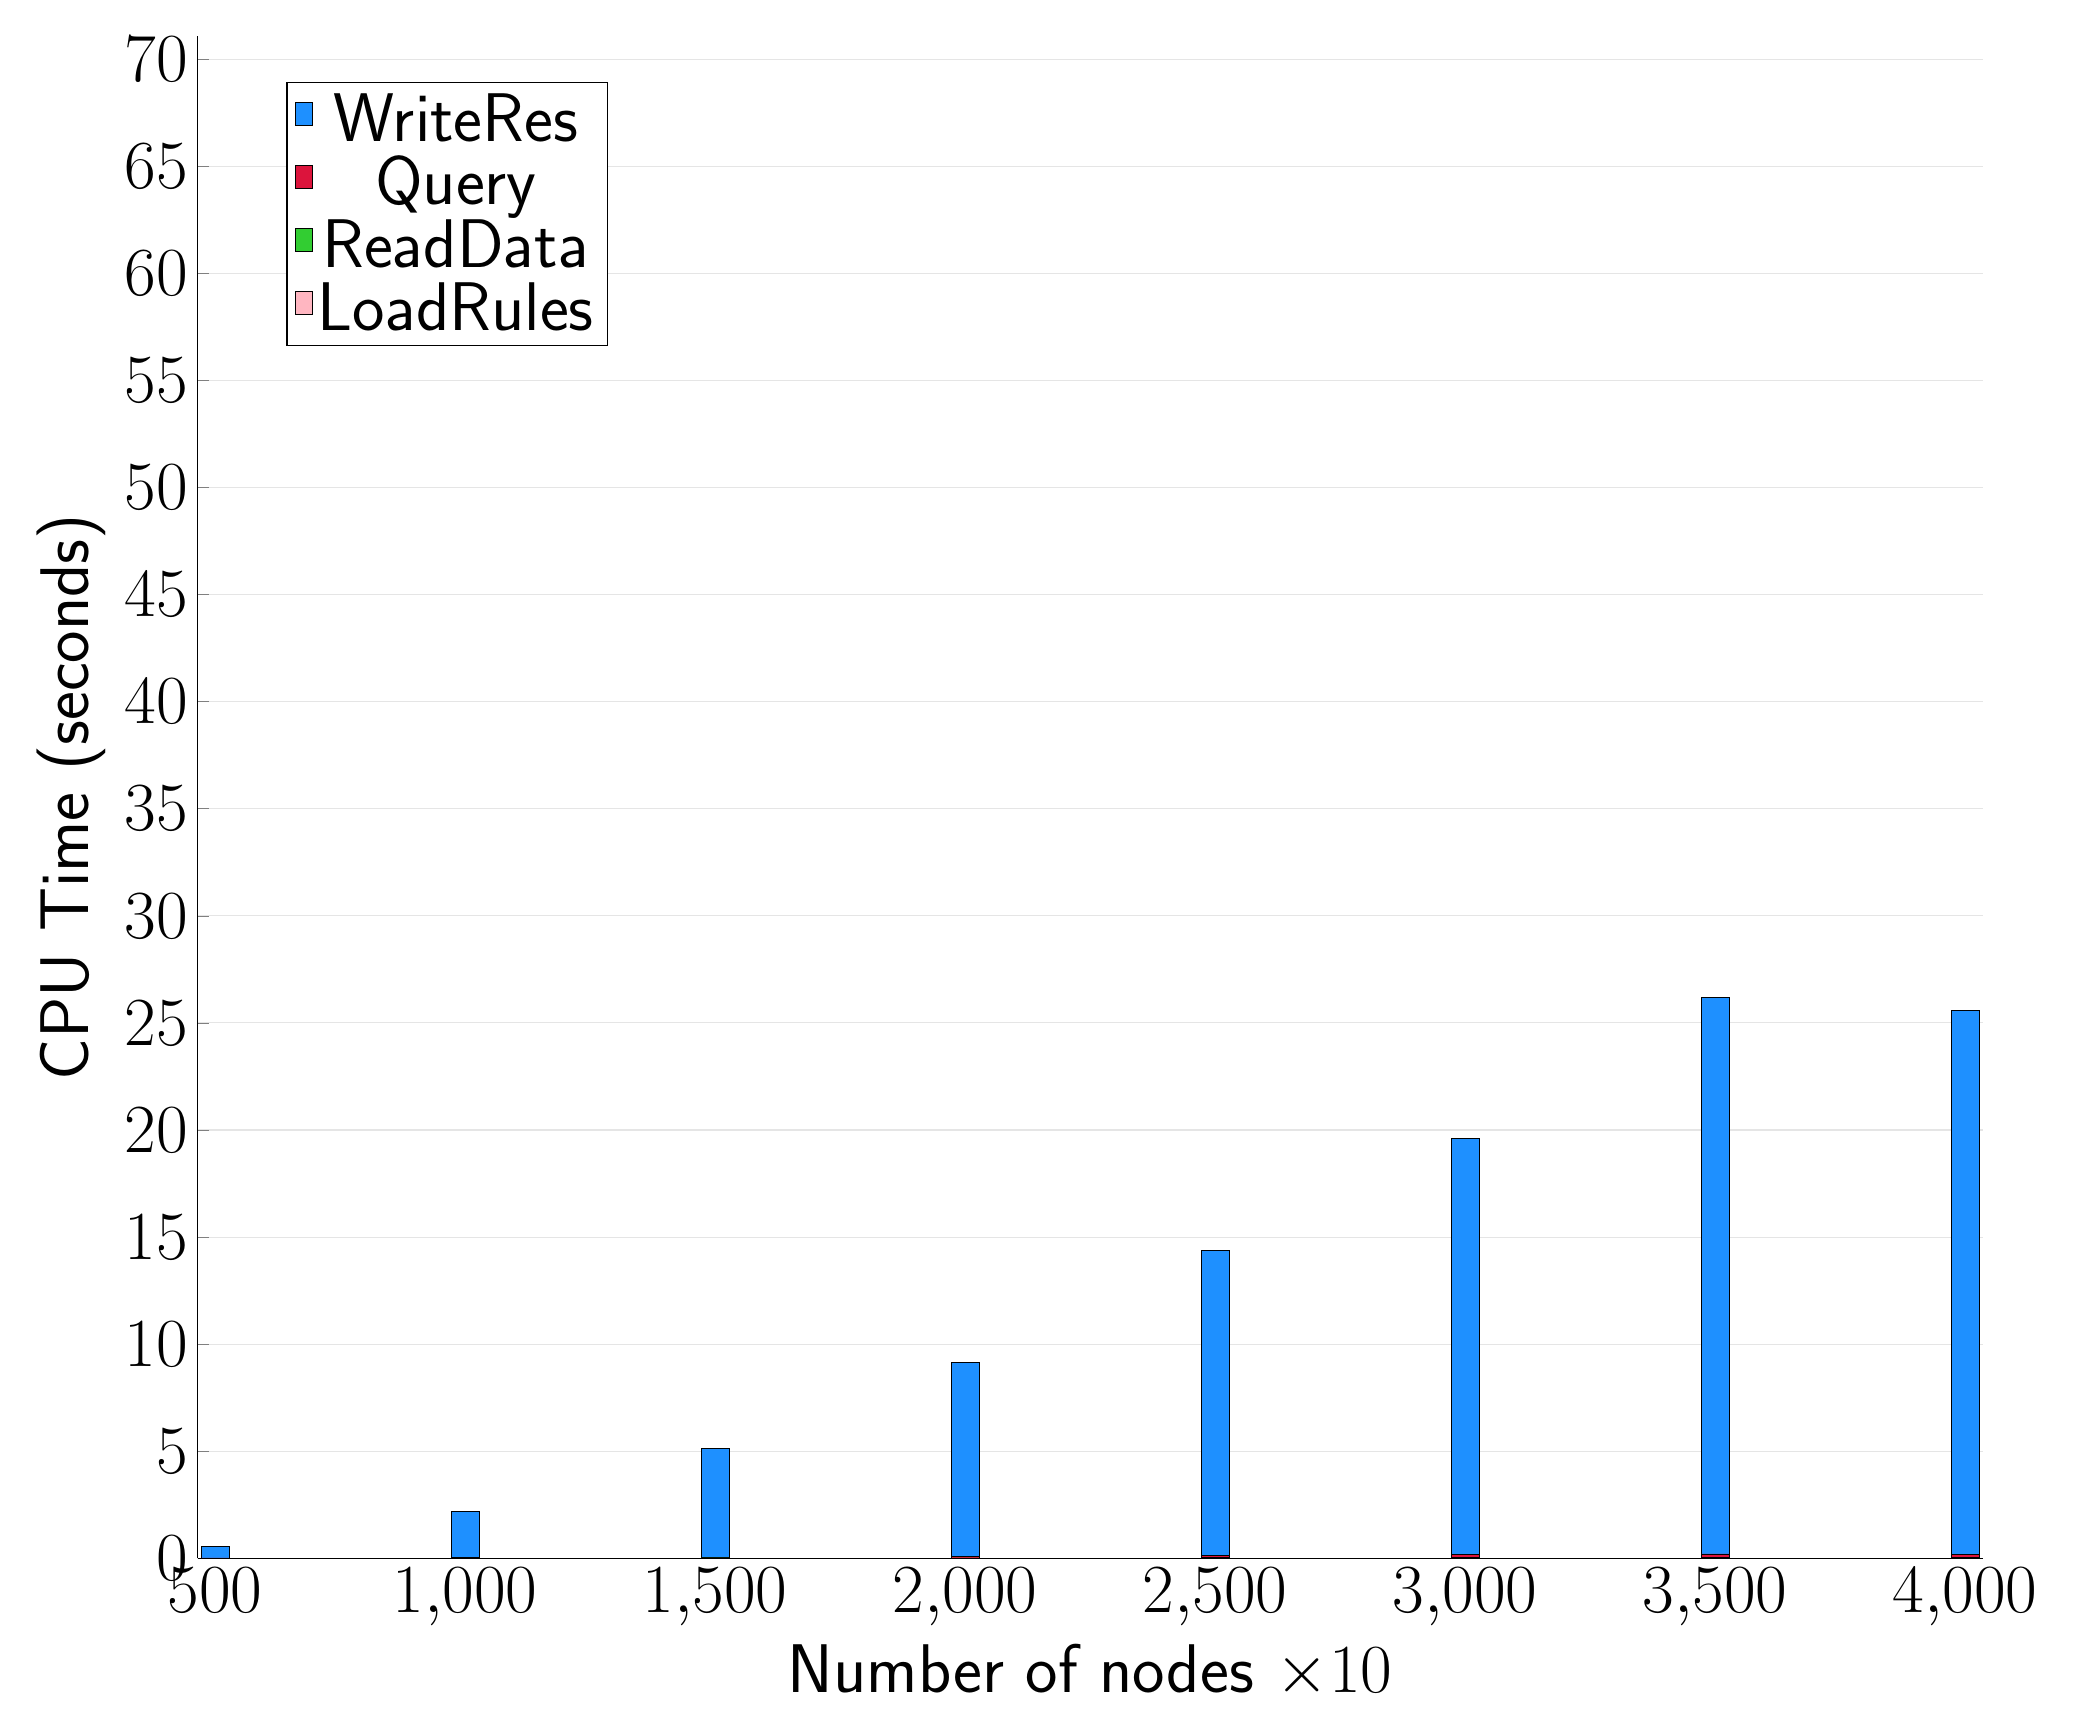
\begin{tikzpicture}
\begin{axis}[
   ybar stacked,
   width=2\textwidth,
   bar width=0.35cm,
   ymajorgrids, tick align=inside,
   major grid style={draw=gray!20},
   xtick=data,
   ymin=0, ymax=71.079008658727,
   axis x line*=bottom,
   axis y line*=left,
   enlarge x limits=0.01,
   legend style={
       at={(0.23, 0.97)},
       anchor=north east,
       legend columns=1,
       font=\Huge,
   },
   ylabel={CPU Time (seconds)},
   xlabel={Number of nodes $\times 10$},
   label style={font=\Huge},
   tick label style={font=\Huge},
]
\addlegendimage{fill=DodgerBlue, draw=black, line width=0.2pt}
\addlegendentry{WriteRes}
\addlegendimage{fill=Crimson, draw=black, line width=0.2pt}
\addlegendentry{Query}
\addlegendimage{fill=LimeGreen, draw=black, line width=0.2pt}
\addlegendentry{ReadData}
\addlegendimage{fill=LightPink, draw=black, line width=0.2pt}
\addlegendentry{LoadRules}
\addplot +[fill=LightPink, draw=black, line width=0.2pt] coordinates {
(500, 0.00547)
(1000, 0.004241000000000003)
(1500, 0.0033830000000000006)
(2000, 0.0018150000000000013)
(2500, 0.004612000000000001)
(3000, 0.002747333333333333)
(3500, 0.003839)
(4000, 0.003145666666666667)
};
\addplot +[fill=LimeGreen, draw=black, line width=0.2pt] coordinates {
(500, 0.010071666666666666)
(1000, 0.014701333333333335)
(1500, 0.021458666666666668)
(2000, 0.023836333333333334)
(2500, 0.03762133333333333)
(3000, 0.04518266666666667)
(3500, 0.049007)
(4000, 0.04779066666666667)
};
\addplot +[fill=Crimson, draw=black, line width=0.2pt] coordinates {
(500, 0.0061226666666666625)
(1000, 0.015392333333333333)
(1500, 0.032133)
(2000, 0.0522)
(2500, 0.090911)
(3000, 0.132877)
(3500, 0.16262466666666667)
(4000, 0.15316466666666667)
};
\addplot +[fill=DodgerBlue, draw=black, line width=0.2pt] coordinates {
(500, 0.5363096666666666)
(1000, 2.1558703333333336)
(1500, 5.097248666666666)
(2000, 9.083624333333335)
(2500, 14.248230999999999)
(3000, 19.436594333333332)
(3500, 25.986491666666666)
(4000, 25.386606999999998)
};
\end{axis}
\end{tikzpicture}

\end{document}
